% Created by tikzDevice version 0.12.3.2 on 2022-02-14 17:14:31
% !TEX encoding = UTF-8 Unicode
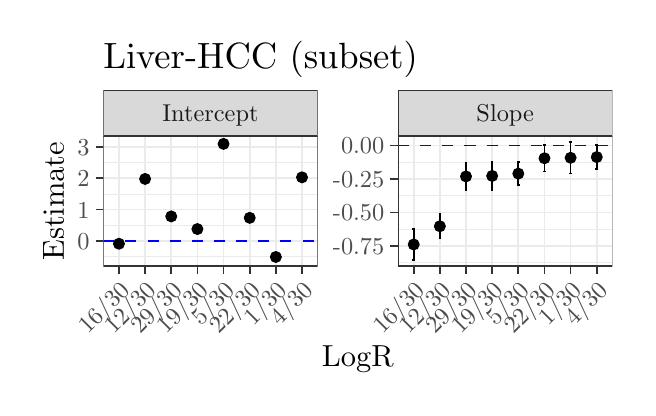
\begin{tikzpicture}[x=1pt,y=1pt]
\definecolor{fillColor}{RGB}{255,255,255}
\path[use as bounding box,fill=fillColor,fill opacity=0.00] (0,0) rectangle (216.81,130.09);
\begin{scope}
\path[clip] (  0.00,  0.00) rectangle (216.81,130.09);
\definecolor{drawColor}{RGB}{255,255,255}
\definecolor{fillColor}{RGB}{255,255,255}

\path[draw=drawColor,line width= 0.6pt,line join=round,line cap=round,fill=fillColor] (  0.00,  0.00) rectangle (216.81,130.09);
\end{scope}
\begin{scope}
\path[clip] ( 27.31, 43.96) rectangle (104.80, 90.86);
\definecolor{fillColor}{RGB}{255,255,255}

\path[fill=fillColor] ( 27.31, 43.96) rectangle (104.80, 90.86);
\definecolor{drawColor}{gray}{0.92}

\path[draw=drawColor,line width= 0.3pt,line join=round] ( 27.31, 47.34) --
	(104.80, 47.34);

\path[draw=drawColor,line width= 0.3pt,line join=round] ( 27.31, 58.67) --
	(104.80, 58.67);

\path[draw=drawColor,line width= 0.3pt,line join=round] ( 27.31, 69.99) --
	(104.80, 69.99);

\path[draw=drawColor,line width= 0.3pt,line join=round] ( 27.31, 81.31) --
	(104.80, 81.31);

\path[draw=drawColor,line width= 0.6pt,line join=round] ( 27.31, 53.01) --
	(104.80, 53.01);

\path[draw=drawColor,line width= 0.6pt,line join=round] ( 27.31, 64.33) --
	(104.80, 64.33);

\path[draw=drawColor,line width= 0.6pt,line join=round] ( 27.31, 75.65) --
	(104.80, 75.65);

\path[draw=drawColor,line width= 0.6pt,line join=round] ( 27.31, 86.97) --
	(104.80, 86.97);

\path[draw=drawColor,line width= 0.6pt,line join=round] ( 32.98, 43.96) --
	( 32.98, 90.86);

\path[draw=drawColor,line width= 0.6pt,line join=round] ( 42.43, 43.96) --
	( 42.43, 90.86);

\path[draw=drawColor,line width= 0.6pt,line join=round] ( 51.88, 43.96) --
	( 51.88, 90.86);

\path[draw=drawColor,line width= 0.6pt,line join=round] ( 61.33, 43.96) --
	( 61.33, 90.86);

\path[draw=drawColor,line width= 0.6pt,line join=round] ( 70.78, 43.96) --
	( 70.78, 90.86);

\path[draw=drawColor,line width= 0.6pt,line join=round] ( 80.23, 43.96) --
	( 80.23, 90.86);

\path[draw=drawColor,line width= 0.6pt,line join=round] ( 89.68, 43.96) --
	( 89.68, 90.86);

\path[draw=drawColor,line width= 0.6pt,line join=round] ( 99.13, 43.96) --
	( 99.13, 90.86);
\definecolor{drawColor}{RGB}{0,0,255}

\path[draw=drawColor,line width= 0.6pt,dash pattern=on 4pt off 4pt ,line join=round] ( 27.31, 53.01) -- (104.80, 53.01);
\definecolor{drawColor}{RGB}{0,0,0}
\definecolor{fillColor}{RGB}{0,0,0}

\path[draw=drawColor,line width= 0.4pt,line join=round,line cap=round,fill=fillColor] ( 89.68, 47.23) circle (  1.96);

\path[draw=drawColor,line width= 0.4pt,line join=round,line cap=round,fill=fillColor] ( 99.13, 76.01) circle (  1.96);

\path[draw=drawColor,line width= 0.4pt,line join=round,line cap=round,fill=fillColor] ( 70.78, 88.10) circle (  1.96);

\path[draw=drawColor,line width= 0.4pt,line join=round,line cap=round,fill=fillColor] ( 42.43, 75.43) circle (  1.96);

\path[draw=drawColor,line width= 0.4pt,line join=round,line cap=round,fill=fillColor] ( 32.98, 52.01) circle (  1.96);

\path[draw=drawColor,line width= 0.4pt,line join=round,line cap=round,fill=fillColor] ( 61.33, 57.32) circle (  1.96);

\path[draw=drawColor,line width= 0.4pt,line join=round,line cap=round,fill=fillColor] ( 80.23, 61.37) circle (  1.96);

\path[draw=drawColor,line width= 0.4pt,line join=round,line cap=round,fill=fillColor] ( 51.88, 61.89) circle (  1.96);

\path[draw=drawColor,line width= 0.6pt,line join=round] ( 89.21, 48.36) --
	( 90.15, 48.36);

\path[draw=drawColor,line width= 0.6pt,line join=round] ( 89.68, 48.36) --
	( 89.68, 46.09);

\path[draw=drawColor,line width= 0.6pt,line join=round] ( 89.21, 46.09) --
	( 90.15, 46.09);

\path[draw=drawColor,line width= 0.6pt,line join=round] ( 98.66, 76.64) --
	( 99.60, 76.64);

\path[draw=drawColor,line width= 0.6pt,line join=round] ( 99.13, 76.64) --
	( 99.13, 75.37);

\path[draw=drawColor,line width= 0.6pt,line join=round] ( 98.66, 75.37) --
	( 99.60, 75.37);

\path[draw=drawColor,line width= 0.6pt,line join=round] ( 70.31, 88.73) --
	( 71.25, 88.73);

\path[draw=drawColor,line width= 0.6pt,line join=round] ( 70.78, 88.73) --
	( 70.78, 87.47);

\path[draw=drawColor,line width= 0.6pt,line join=round] ( 70.31, 87.47) --
	( 71.25, 87.47);

\path[draw=drawColor,line width= 0.6pt,line join=round] ( 41.96, 76.44) --
	( 42.91, 76.44);

\path[draw=drawColor,line width= 0.6pt,line join=round] ( 42.43, 76.44) --
	( 42.43, 74.43);

\path[draw=drawColor,line width= 0.6pt,line join=round] ( 41.96, 74.43) --
	( 42.91, 74.43);

\path[draw=drawColor,line width= 0.6pt,line join=round] ( 32.51, 53.51) --
	( 33.46, 53.51);

\path[draw=drawColor,line width= 0.6pt,line join=round] ( 32.98, 53.51) --
	( 32.98, 50.52);

\path[draw=drawColor,line width= 0.6pt,line join=round] ( 32.51, 50.52) --
	( 33.46, 50.52);

\path[draw=drawColor,line width= 0.6pt,line join=round] ( 60.86, 58.13) --
	( 61.80, 58.13);

\path[draw=drawColor,line width= 0.6pt,line join=round] ( 61.33, 58.13) --
	( 61.33, 56.51);

\path[draw=drawColor,line width= 0.6pt,line join=round] ( 60.86, 56.51) --
	( 61.80, 56.51);

\path[draw=drawColor,line width= 0.6pt,line join=round] ( 79.76, 62.16) --
	( 80.70, 62.16);

\path[draw=drawColor,line width= 0.6pt,line join=round] ( 80.23, 62.16) --
	( 80.23, 60.59);

\path[draw=drawColor,line width= 0.6pt,line join=round] ( 79.76, 60.59) --
	( 80.70, 60.59);

\path[draw=drawColor,line width= 0.6pt,line join=round] ( 51.41, 62.69) --
	( 52.35, 62.69);

\path[draw=drawColor,line width= 0.6pt,line join=round] ( 51.88, 62.69) --
	( 51.88, 61.09);

\path[draw=drawColor,line width= 0.6pt,line join=round] ( 51.41, 61.09) --
	( 52.35, 61.09);
\definecolor{drawColor}{gray}{0.20}

\path[draw=drawColor,line width= 0.6pt,line join=round,line cap=round] ( 27.31, 43.96) rectangle (104.80, 90.86);
\end{scope}
\begin{scope}
\path[clip] (133.82, 43.96) rectangle (211.31, 90.86);
\definecolor{fillColor}{RGB}{255,255,255}

\path[fill=fillColor] (133.82, 43.96) rectangle (211.31, 90.86);
\definecolor{drawColor}{gray}{0.92}

\path[draw=drawColor,line width= 0.3pt,line join=round] (133.82, 45.12) --
	(211.31, 45.12);

\path[draw=drawColor,line width= 0.3pt,line join=round] (133.82, 57.22) --
	(211.31, 57.22);

\path[draw=drawColor,line width= 0.3pt,line join=round] (133.82, 69.32) --
	(211.31, 69.32);

\path[draw=drawColor,line width= 0.3pt,line join=round] (133.82, 81.43) --
	(211.31, 81.43);

\path[draw=drawColor,line width= 0.6pt,line join=round] (133.82, 51.17) --
	(211.31, 51.17);

\path[draw=drawColor,line width= 0.6pt,line join=round] (133.82, 63.27) --
	(211.31, 63.27);

\path[draw=drawColor,line width= 0.6pt,line join=round] (133.82, 75.37) --
	(211.31, 75.37);

\path[draw=drawColor,line width= 0.6pt,line join=round] (133.82, 87.48) --
	(211.31, 87.48);

\path[draw=drawColor,line width= 0.6pt,line join=round] (139.49, 43.96) --
	(139.49, 90.86);

\path[draw=drawColor,line width= 0.6pt,line join=round] (148.94, 43.96) --
	(148.94, 90.86);

\path[draw=drawColor,line width= 0.6pt,line join=round] (158.39, 43.96) --
	(158.39, 90.86);

\path[draw=drawColor,line width= 0.6pt,line join=round] (167.84, 43.96) --
	(167.84, 90.86);

\path[draw=drawColor,line width= 0.6pt,line join=round] (177.29, 43.96) --
	(177.29, 90.86);

\path[draw=drawColor,line width= 0.6pt,line join=round] (186.74, 43.96) --
	(186.74, 90.86);

\path[draw=drawColor,line width= 0.6pt,line join=round] (196.19, 43.96) --
	(196.19, 90.86);

\path[draw=drawColor,line width= 0.6pt,line join=round] (205.64, 43.96) --
	(205.64, 90.86);
\definecolor{drawColor}{RGB}{0,0,255}

\path[draw=drawColor,line width= 0.6pt,dash pattern=on 4pt off 4pt ,line join=round] (133.82, 87.48) -- (211.31, 87.48);
\definecolor{drawColor}{RGB}{0,0,0}
\definecolor{fillColor}{RGB}{0,0,0}

\path[draw=drawColor,line width= 0.4pt,line join=round,line cap=round,fill=fillColor] (196.19, 83.07) circle (  1.96);

\path[draw=drawColor,line width= 0.4pt,line join=round,line cap=round,fill=fillColor] (205.64, 83.33) circle (  1.96);

\path[draw=drawColor,line width= 0.4pt,line join=round,line cap=round,fill=fillColor] (177.29, 77.35) circle (  1.96);

\path[draw=drawColor,line width= 0.4pt,line join=round,line cap=round,fill=fillColor] (148.94, 58.33) circle (  1.96);

\path[draw=drawColor,line width= 0.4pt,line join=round,line cap=round,fill=fillColor] (139.49, 51.75) circle (  1.96);

\path[draw=drawColor,line width= 0.4pt,line join=round,line cap=round,fill=fillColor] (167.84, 76.51) circle (  1.96);

\path[draw=drawColor,line width= 0.4pt,line join=round,line cap=round,fill=fillColor] (186.74, 82.90) circle (  1.96);

\path[draw=drawColor,line width= 0.4pt,line join=round,line cap=round,fill=fillColor] (158.39, 76.34) circle (  1.96);

\path[draw=drawColor,line width= 0.6pt,line join=round] (195.72, 88.73) --
	(196.66, 88.73);

\path[draw=drawColor,line width= 0.6pt,line join=round] (196.19, 88.73) --
	(196.19, 77.42);

\path[draw=drawColor,line width= 0.6pt,line join=round] (195.72, 77.42) --
	(196.66, 77.42);

\path[draw=drawColor,line width= 0.6pt,line join=round] (205.17, 87.63) --
	(206.11, 87.63);

\path[draw=drawColor,line width= 0.6pt,line join=round] (205.64, 87.63) --
	(205.64, 79.03);

\path[draw=drawColor,line width= 0.6pt,line join=round] (205.17, 79.03) --
	(206.11, 79.03);

\path[draw=drawColor,line width= 0.6pt,line join=round] (176.82, 81.47) --
	(177.76, 81.47);

\path[draw=drawColor,line width= 0.6pt,line join=round] (177.29, 81.47) --
	(177.29, 73.23);

\path[draw=drawColor,line width= 0.6pt,line join=round] (176.82, 73.23) --
	(177.76, 73.23);

\path[draw=drawColor,line width= 0.6pt,line join=round] (148.47, 62.70) --
	(149.42, 62.70);

\path[draw=drawColor,line width= 0.6pt,line join=round] (148.94, 62.70) --
	(148.94, 53.95);

\path[draw=drawColor,line width= 0.6pt,line join=round] (148.47, 53.95) --
	(149.42, 53.95);

\path[draw=drawColor,line width= 0.6pt,line join=round] (139.02, 57.41) --
	(139.97, 57.41);

\path[draw=drawColor,line width= 0.6pt,line join=round] (139.49, 57.41) --
	(139.49, 46.09);

\path[draw=drawColor,line width= 0.6pt,line join=round] (139.02, 46.09) --
	(139.97, 46.09);

\path[draw=drawColor,line width= 0.6pt,line join=round] (167.37, 81.69) --
	(168.31, 81.69);

\path[draw=drawColor,line width= 0.6pt,line join=round] (167.84, 81.69) --
	(167.84, 71.34);

\path[draw=drawColor,line width= 0.6pt,line join=round] (167.37, 71.34) --
	(168.31, 71.34);

\path[draw=drawColor,line width= 0.6pt,line join=round] (186.27, 87.74) --
	(187.21, 87.74);

\path[draw=drawColor,line width= 0.6pt,line join=round] (186.74, 87.74) --
	(186.74, 78.06);

\path[draw=drawColor,line width= 0.6pt,line join=round] (186.27, 78.06) --
	(187.21, 78.06);

\path[draw=drawColor,line width= 0.6pt,line join=round] (157.92, 81.31) --
	(158.86, 81.31);

\path[draw=drawColor,line width= 0.6pt,line join=round] (158.39, 81.31) --
	(158.39, 71.38);

\path[draw=drawColor,line width= 0.6pt,line join=round] (157.92, 71.38) --
	(158.86, 71.38);
\definecolor{drawColor}{gray}{0.20}

\path[draw=drawColor,line width= 0.6pt,line join=round,line cap=round] (133.82, 43.96) rectangle (211.31, 90.86);
\end{scope}
\begin{scope}
\path[clip] ( 27.31, 90.86) rectangle (104.80,107.43);
\definecolor{drawColor}{gray}{0.20}
\definecolor{fillColor}{gray}{0.85}

\path[draw=drawColor,line width= 0.6pt,line join=round,line cap=round,fill=fillColor] ( 27.31, 90.86) rectangle (104.80,107.43);
\definecolor{drawColor}{gray}{0.10}

\node[text=drawColor,anchor=base,inner sep=0pt, outer sep=0pt, scale=  0.88] at ( 66.06, 96.11) {Intercept};
\end{scope}
\begin{scope}
\path[clip] (133.82, 90.86) rectangle (211.31,107.43);
\definecolor{drawColor}{gray}{0.20}
\definecolor{fillColor}{gray}{0.85}

\path[draw=drawColor,line width= 0.6pt,line join=round,line cap=round,fill=fillColor] (133.82, 90.86) rectangle (211.31,107.43);
\definecolor{drawColor}{gray}{0.10}

\node[text=drawColor,anchor=base,inner sep=0pt, outer sep=0pt, scale=  0.88] at (172.57, 96.11) {Slope};
\end{scope}
\begin{scope}
\path[clip] (  0.00,  0.00) rectangle (216.81,130.09);
\definecolor{drawColor}{gray}{0.20}

\path[draw=drawColor,line width= 0.6pt,line join=round] ( 32.98, 41.21) --
	( 32.98, 43.96);

\path[draw=drawColor,line width= 0.6pt,line join=round] ( 42.43, 41.21) --
	( 42.43, 43.96);

\path[draw=drawColor,line width= 0.6pt,line join=round] ( 51.88, 41.21) --
	( 51.88, 43.96);

\path[draw=drawColor,line width= 0.6pt,line join=round] ( 61.33, 41.21) --
	( 61.33, 43.96);

\path[draw=drawColor,line width= 0.6pt,line join=round] ( 70.78, 41.21) --
	( 70.78, 43.96);

\path[draw=drawColor,line width= 0.6pt,line join=round] ( 80.23, 41.21) --
	( 80.23, 43.96);

\path[draw=drawColor,line width= 0.6pt,line join=round] ( 89.68, 41.21) --
	( 89.68, 43.96);

\path[draw=drawColor,line width= 0.6pt,line join=round] ( 99.13, 41.21) --
	( 99.13, 43.96);
\end{scope}
\begin{scope}
\path[clip] (  0.00,  0.00) rectangle (216.81,130.09);
\definecolor{drawColor}{gray}{0.30}

\node[text=drawColor,rotate= 45.00,anchor=base east,inner sep=0pt, outer sep=0pt, scale=  0.88] at ( 37.27, 34.73) {16/30};

\node[text=drawColor,rotate= 45.00,anchor=base east,inner sep=0pt, outer sep=0pt, scale=  0.88] at ( 46.72, 34.73) {12/30};

\node[text=drawColor,rotate= 45.00,anchor=base east,inner sep=0pt, outer sep=0pt, scale=  0.88] at ( 56.17, 34.73) {29/30};

\node[text=drawColor,rotate= 45.00,anchor=base east,inner sep=0pt, outer sep=0pt, scale=  0.88] at ( 65.62, 34.73) {19/30};

\node[text=drawColor,rotate= 45.00,anchor=base east,inner sep=0pt, outer sep=0pt, scale=  0.88] at ( 75.07, 34.73) {5/30};

\node[text=drawColor,rotate= 45.00,anchor=base east,inner sep=0pt, outer sep=0pt, scale=  0.88] at ( 84.52, 34.73) {22/30};

\node[text=drawColor,rotate= 45.00,anchor=base east,inner sep=0pt, outer sep=0pt, scale=  0.88] at ( 93.97, 34.73) {1/30};

\node[text=drawColor,rotate= 45.00,anchor=base east,inner sep=0pt, outer sep=0pt, scale=  0.88] at (103.42, 34.73) {4/30};
\end{scope}
\begin{scope}
\path[clip] (  0.00,  0.00) rectangle (216.81,130.09);
\definecolor{drawColor}{gray}{0.20}

\path[draw=drawColor,line width= 0.6pt,line join=round] (139.49, 41.21) --
	(139.49, 43.96);

\path[draw=drawColor,line width= 0.6pt,line join=round] (148.94, 41.21) --
	(148.94, 43.96);

\path[draw=drawColor,line width= 0.6pt,line join=round] (158.39, 41.21) --
	(158.39, 43.96);

\path[draw=drawColor,line width= 0.6pt,line join=round] (167.84, 41.21) --
	(167.84, 43.96);

\path[draw=drawColor,line width= 0.6pt,line join=round] (177.29, 41.21) --
	(177.29, 43.96);

\path[draw=drawColor,line width= 0.6pt,line join=round] (186.74, 41.21) --
	(186.74, 43.96);

\path[draw=drawColor,line width= 0.6pt,line join=round] (196.19, 41.21) --
	(196.19, 43.96);

\path[draw=drawColor,line width= 0.6pt,line join=round] (205.64, 41.21) --
	(205.64, 43.96);
\end{scope}
\begin{scope}
\path[clip] (  0.00,  0.00) rectangle (216.81,130.09);
\definecolor{drawColor}{gray}{0.30}

\node[text=drawColor,rotate= 45.00,anchor=base east,inner sep=0pt, outer sep=0pt, scale=  0.88] at (143.78, 34.73) {16/30};

\node[text=drawColor,rotate= 45.00,anchor=base east,inner sep=0pt, outer sep=0pt, scale=  0.88] at (153.23, 34.73) {12/30};

\node[text=drawColor,rotate= 45.00,anchor=base east,inner sep=0pt, outer sep=0pt, scale=  0.88] at (162.68, 34.73) {29/30};

\node[text=drawColor,rotate= 45.00,anchor=base east,inner sep=0pt, outer sep=0pt, scale=  0.88] at (172.13, 34.73) {19/30};

\node[text=drawColor,rotate= 45.00,anchor=base east,inner sep=0pt, outer sep=0pt, scale=  0.88] at (181.58, 34.73) {5/30};

\node[text=drawColor,rotate= 45.00,anchor=base east,inner sep=0pt, outer sep=0pt, scale=  0.88] at (191.03, 34.73) {22/30};

\node[text=drawColor,rotate= 45.00,anchor=base east,inner sep=0pt, outer sep=0pt, scale=  0.88] at (200.48, 34.73) {1/30};

\node[text=drawColor,rotate= 45.00,anchor=base east,inner sep=0pt, outer sep=0pt, scale=  0.88] at (209.93, 34.73) {4/30};
\end{scope}
\begin{scope}
\path[clip] (  0.00,  0.00) rectangle (216.81,130.09);
\definecolor{drawColor}{gray}{0.30}

\node[text=drawColor,anchor=base east,inner sep=0pt, outer sep=0pt, scale=  0.88] at (128.87, 48.14) {-0.75};

\node[text=drawColor,anchor=base east,inner sep=0pt, outer sep=0pt, scale=  0.88] at (128.87, 60.24) {-0.50};

\node[text=drawColor,anchor=base east,inner sep=0pt, outer sep=0pt, scale=  0.88] at (128.87, 72.34) {-0.25};

\node[text=drawColor,anchor=base east,inner sep=0pt, outer sep=0pt, scale=  0.88] at (128.87, 84.45) {0.00};
\end{scope}
\begin{scope}
\path[clip] (  0.00,  0.00) rectangle (216.81,130.09);
\definecolor{drawColor}{gray}{0.20}

\path[draw=drawColor,line width= 0.6pt,line join=round] (131.07, 51.17) --
	(133.82, 51.17);

\path[draw=drawColor,line width= 0.6pt,line join=round] (131.07, 63.27) --
	(133.82, 63.27);

\path[draw=drawColor,line width= 0.6pt,line join=round] (131.07, 75.37) --
	(133.82, 75.37);

\path[draw=drawColor,line width= 0.6pt,line join=round] (131.07, 87.48) --
	(133.82, 87.48);
\end{scope}
\begin{scope}
\path[clip] (  0.00,  0.00) rectangle (216.81,130.09);
\definecolor{drawColor}{gray}{0.30}

\node[text=drawColor,anchor=base east,inner sep=0pt, outer sep=0pt, scale=  0.88] at ( 22.36, 49.97) {0};

\node[text=drawColor,anchor=base east,inner sep=0pt, outer sep=0pt, scale=  0.88] at ( 22.36, 61.30) {1};

\node[text=drawColor,anchor=base east,inner sep=0pt, outer sep=0pt, scale=  0.88] at ( 22.36, 72.62) {2};

\node[text=drawColor,anchor=base east,inner sep=0pt, outer sep=0pt, scale=  0.88] at ( 22.36, 83.94) {3};
\end{scope}
\begin{scope}
\path[clip] (  0.00,  0.00) rectangle (216.81,130.09);
\definecolor{drawColor}{gray}{0.20}

\path[draw=drawColor,line width= 0.6pt,line join=round] ( 24.56, 53.01) --
	( 27.31, 53.01);

\path[draw=drawColor,line width= 0.6pt,line join=round] ( 24.56, 64.33) --
	( 27.31, 64.33);

\path[draw=drawColor,line width= 0.6pt,line join=round] ( 24.56, 75.65) --
	( 27.31, 75.65);

\path[draw=drawColor,line width= 0.6pt,line join=round] ( 24.56, 86.97) --
	( 27.31, 86.97);
\end{scope}
\begin{scope}
\path[clip] (  0.00,  0.00) rectangle (216.81,130.09);
\definecolor{drawColor}{RGB}{0,0,0}

\node[text=drawColor,anchor=base,inner sep=0pt, outer sep=0pt, scale=  1.10] at (119.31,  7.64) {LogR};
\end{scope}
\begin{scope}
\path[clip] (  0.00,  0.00) rectangle (216.81,130.09);
\definecolor{drawColor}{RGB}{0,0,0}

\node[text=drawColor,rotate= 90.00,anchor=base,inner sep=0pt, outer sep=0pt, scale=  1.10] at ( 13.08, 67.41) {Estimate};
\end{scope}
\begin{scope}
\path[clip] (  0.00,  0.00) rectangle (216.81,130.09);
\definecolor{drawColor}{RGB}{0,0,0}

\node[text=drawColor,anchor=base west,inner sep=0pt, outer sep=0pt, scale=  1.32] at ( 27.31,115.49) {Liver-HCC (subset)};
\end{scope}
\end{tikzpicture}
